\documentclass[11pt,a4paper]{article}

\usepackage[T1]{fontenc}
\usepackage{lmodern}
\usepackage[margin=0.95in]{geometry}
\usepackage{amsmath,amssymb,amsthm,mathtools}
\usepackage{graphicx}
\usepackage{booktabs}
\usepackage{array}
\usepackage{xcolor}
\usepackage{hyperref}
\usepackage{microtype}
\usepackage{enumitem}
\usepackage{caption}
\usepackage{xurl}

\emergencystretch=2.2em

\hypersetup{
  colorlinks=true,
  linkcolor=blue!65!black,
  citecolor=green!45!black,
  urlcolor=blue!65!black
}

\newtheorem{theorem}{Theorem}[section]
\newtheorem{proposition}[theorem]{Proposition}
\newtheorem{lemma}[theorem]{Lemma}
\newtheorem{corollary}[theorem]{Corollary}
\theoremstyle{definition}
\newtheorem{definition}[theorem]{Definition}
\theoremstyle{remark}
\newtheorem{remark}[theorem]{Remark}

\newcommand{\F}{\mathbb{F}}
\newcommand{\Z}{\mathbb{Z}}
\newcommand{\Q}{\mathbb{Q}}
\newcommand{\R}{\mathbb{R}}
\newcommand{\STAB}{\mathrm{STAB}}
\newcommand{\RoM}{\mathcal{R}}
\newcommand{\Pauli}{\mathcal{P}}
\newcommand{\Tr}{\operatorname{Tr}}
\newcommand{\Code}[1]{{\small\texttt{#1}}}

\title{\textbf{Symplectic Clique-Cover Duality, Signed Frustration Atoms, and Zero-Enumeration Exact-$\Q$ Robustness-of-Magic Certificates for Multi-Qubit Quantum States}}

\author{
  Lluis Eriksson\thanks{Independent researcher (Sweden). Prepared with AI assistance (Google Antigravity). Code, Lean~4 proofs, and exact-$\Q$ certificates: \url{https://github.com/lluiseriksson/symplectic-magic-certificates} (MIT license).}
}
\date{November 24, 2026}

\begin{document}
\maketitle

\begin{abstract}
Certifying non-stabilizerness (``quantum magic'') and bounding the Robustness of Magic $\RoM(\rho)$ for multi-qubit mixed states is central to fault-tolerant quantum computation, yet exact linear-programming membership in the stabilizer polytope $\STAB_n$ encounters a $2^{\Theta(n^2)}$ vertex wall beyond $n \approx 5$ qubits, while pure-state monotones such as Stabilizer R\'enyi Entropy fail for mixed states. Building on recent worst-case random access code (RAC) frameworks (Zamora, Nov 2026), we introduce a zero-enumeration, zero-floating-point-trust dual certification framework based on two elementary symplectic atoms over $\F_2^{2n}$: \emph{anticommuting Pauli cliques} ($C \in [-1, +1]$ on $\STAB_n$) and \emph{signed frustrated commuting triples} ($F \in [-3, +1]$ via $\F_2$-subgroup closure, strictly below their unsigned independence number~$3$). First, we prove the \textbf{Symplectic Atom-Cover and Chv\'atal--Gomory Rounding Theorem} (Theorem~\ref{thm:atom-cover}): any conical decomposition $W = \sum_j y_j C_j + \sum_\ell z_\ell F_\ell$ ($y_j, z_\ell \in \Q_{\ge 0}$) yields exact stabilizer bounds $[-\hat{\beta}_-, +\hat{\beta}_+]$ (sharpened by integer floors $\lfloor \beta_\pm \rfloor$ whenever $W$ has integer weights), certifying exact mixed-state Robustness of Magic $\RoM(\rho) \ge 1 + 2(\Tr(W\rho) - \hat{\beta}_+)/(\hat{\beta}_+ + \hat{\beta}_-)$ and depolarizing noise tolerance $p_{\mathrm{cert}} = 1 - \hat{\beta}_+/\Tr(W\rho)$ without enumerating $\STAB_n$. Second, we establish exact worst-case RAC bounds (Theorem~\ref{thm:rac}), including $B_{\mathrm{wc}}(\sigma) \le 1/(2^n + 1)$ on all non-identity Paulis $\Pauli_n \setminus \{I\}$. Third, we prove an \textbf{exponential separation over the standard Pauli $\ell_1$-norm bound} (Theorem~\ref{thm:majorana}): on the rank-$2^{n-1}$ mixed Majorana-clique state $\rho_{K_{2n+1}}$ (purity $2^{1-n} \to 0$), Pauli $\ell_1$-norm decays as $(1+\sqrt{2n+1})/2^n \to 0$ (blind for all $n \ge 2$), whereas our $(2n+1)$-Pauli clique certificate proves $\RoM(\rho_{K_{2n+1}}) \ge \sqrt{2n+1}$ ($p_{\mathrm{cert}} = 1 - 1/\sqrt{2n+1}$), reaching $\RoM \ge 8.062$ and $p_{\mathrm{cert}} = 87.6\%$ at $n = 32$ qubits (bypassing $|\STAB_{32}| \approx 10^{168.95}$) in under $2\,\mathrm{ms}$. Fourth, we resolve the stabilizer-marginal problem for arbitrary $n$-qubit $W$-states (Theorem~\ref{thm:w-state}): every 2-qubit marginal of $|W_n\rangle$ lies inside $\STAB_2$, yet the three weight-$\le 2$ Paulis $\{Z_0, X_0 X_1, Y_0 Y_2\}$ certify $\RoM(|W_n\rangle) \ge \RoM(\rho^{(3)}_{W_n}) \ge 1 + 2/n$ for all $n \ge 3$. Fifth, we prove a \textbf{strict 3-tier hierarchy} for fixed-witness stabilizer ceiling certification (Theorem~\ref{thm:hierarchy}) separating Signed Frustration Atoms $>$ Chv\'atal--Gomory Clique Covers ($C_5$ pentagram) $>$ Single Cliques ($|\mathrm{CCZ}\rangle$, $K_{2n+1}$) $>$ Pauli $\ell_1$-Norm, paired with an exact \textbf{Subset-Dominance Dichotomy} (Proposition~\ref{prop:subset-dominance}) proving that because every frustrated commuting triple obeys $F_\ell \preceq +I$ on all quantum states, Tiers~1--2 strictly dominate non-CG-rounded Tier~3 whenever individual Pauli expectations can be re-weighted into sub-witnesses, whereas Tier~3 strictly lowers the stabilizer ceiling $\hat{\beta}_+(W)$ of fixed signed witnesses below every unsigned graph invariant. All 16 core theorems are mechanized in zero-dependency Lean~4 (\Code{v4.35.0}, \textbf{0~\Code{sorry}}, \textbf{0~\Code{Classical.choice}}), and our exact-$\Q$ verifier validates 9/9 published certificates ($n = 1\dots 32$) while rejecting 28/28 live adversarial forgery, canonical-parser, and type-injection attacks.
\end{abstract}

\section{Introduction}
\label{sec:intro}

By the Gottesman--Knill theorem \cite{AaronsonGottesman2004}, Clifford circuits acting on stabilizer states are efficiently classically simulable; universal fault-tolerant quantum computation requires \emph{non-stabilizerness} (``magic'') \cite{BravyiKitaev2005,Veitch2014Resource}. The canonical operational quantifier of mixed-state magic is the \emph{Robustness of Magic} (RoM) \cite{HowardCampbell2017},
\begin{equation}
  \RoM(\rho) \;:=\; \min\left\{\sum_i |x_i| \;:\; \rho = \sum_i x_i |\phi_i\rangle\langle\phi_i|,\; |\phi_i\rangle \in \mathcal{S}_n,\; \sum_i x_i = 1\right\},
  \label{eq:rom-def}
\end{equation}
which directly governs quasiprobability simulation overhead and magic-state distillation thresholds \cite{HowardCampbell2017,SeddonCampbell2019}. However, because the number of pure $n$-qubit stabilizer states grows super-exponentially as
\begin{equation}
  |\mathcal{S}_n| \;=\; 2^n \prod_{j=1}^n (2^j + 1) \;=\; 2^{\Theta(n^2)},
  \label{eq:stab-count}
\end{equation}
exact primal/dual linear programming over the stabilizer polytope $\STAB_n = \operatorname{conv}\{|\phi\rangle\langle\phi| : |\phi\rangle \in \mathcal{S}_n\}$ becomes intractable beyond $n = 5$ qubits even after exploiting Clifford symmetries \cite{HeinrichGross2019}. Conversely, scalable pure-state magic monotones such as Stabilizer R\'enyi Entropy (SRE) \cite{Leone2022SRE} are strictly inapplicable to certifying mixed-state non-stabilizerness (convex mixtures of stabilizer states have positive SRE), and the classic Pauli $\ell_1$-norm lower bound $\RoM(\rho) \ge 2^{-n} \sum_{P \in \Pauli_n} |\Tr(P\rho)|$ \cite{HowardCampbell2017} requires measuring all $4^n - 1$ non-identity Paulis and collapses exponentially on low-purity mixed states.

In November 2026, Zamora \cite{Zamora2026RAC} introduced a semi-device-independent framework certifying multi-qubit non-stabilizerness via \emph{worst-case random access codes} (RACs) with partially characterized Pauli measurements, proving a \emph{stabilizer pigeonhole criterion} for pure states (applied to $n$-qubit $W$-states using 8 preparations and 3 measurement settings), constructing stabilizer-marginal paradoxes, and bounding worst-case biases for mixed stabilizer preparations. This work raises three sharp foundational questions:
\begin{enumerate}[leftmargin=1.8em,itemsep=2pt]
  \item \textbf{Zero-Enumeration Dual Certificates for Mixed-State RoM:} Can we construct polynomial-size, exact-$\Q$, machine-verifiable dual witnesses of $\STAB_n$ that certify quantitative Robustness of Magic lower bounds $\RoM(\rho) > 1$ and depolarizing noise thresholds for \emph{mixed} states up to dozens of qubits without enumerating $\STAB_n$?
  \item \textbf{Going Beyond Single Cliques and Unsigned Anticommutation Graphs:} Can integer-programming cuts (Chv\'atal--Gomory rounding \cite{Schrijver1986}) and \emph{signed symplectic group closure} strictly beat both single-clique bounds ($1/\omega$) and \emph{every} unsigned graph-theoretic bound ($\alpha_w(G_{\mathrm{anti}})$)?
  \item \textbf{Formal Machine-Checked Soundness:} Can the entire symplectic duality, integer-floor tightening, shifted robustness inequality, and noise-threshold chain be mechanized in Lean~4 \cite{deMoura2021Lean4} and paired with a zero-floating-point-trust certificate verifier?
\end{enumerate}

We answer all three questions affirmatively via a unified three-tier hierarchy of symplectic dual atoms, 16 zero-dependency Lean~4 theorems, and 9 exact-$\Q$ certificates spanning $n = 1$ to $n = 32$ qubits.

\section{Symplectic Dual Atoms and Exact Robustness Bounds}
\label{sec:theory}

\subsection{Symplectic Pauli Algebra over \texorpdfstring{$\F_2^{2n}$}{F2\textasciicircum(2n)}}
Every $n$-qubit Hermitian Pauli operator $P(u)$ ($u = (x, z) \in \F_2^n \times \F_2^n$) is defined as $P(x, z) = i^{|x \wedge z|} X^x Z^z$, where $|x \wedge z| = \sum_{k=0}^{n-1} x_k z_k$. Two Paulis $P(u), P(v)$ satisfy $P(u)P(v) = (-1)^{\omega(u, v)} P(v)P(u)$, where the binary symplectic inner product is
\begin{equation}
  \omega\bigl((x_1, z_1),\, (x_2, z_2)\bigr) \;=\; \sum_{k=0}^{n-1} \bigl(x_{1,k} z_{2,k} + z_{1,k} x_{2,k}\bigr) \pmod 2.
  \label{eq:symp}
\end{equation}
We verify its alternating, symmetric, and bilinear properties directly in Lean~4 (\Code{symp\_self\_zero}, \Code{symp\_comm}, \Code{symp\_bilinear\_left}). When $\omega(u, v) = 0$, the product is Hermitian up to a real sign: $P(u) P(v) = \sigma(u, v)\, P(u \oplus v)$ with $\sigma(u, v) \in \{-1, +1\}$.

Every pure $n$-qubit stabilizer state $|\phi\rangle \in \mathcal{S}_n$ is uniquely specified by a maximal abelian (Lagrangian) subgroup $S_\phi \subset \Pauli_n$ of cardinality $|S_\phi| = 2^n$ (not containing $-I$), such that $\langle\phi|P(u)|\phi\rangle \in \{-1, +1\}$ for $u \in S_\phi$ and $0$ otherwise. Crucially, the support $S_\phi$ satisfies two algebraic constraints simultaneously: (i)~\emph{pairwise commutation} ($\omega(u, v) = 0$ for all $u, v \in S_\phi$), and (ii)~\emph{signed abelian group closure} (if $u, v \in S_\phi$, then $u \oplus v \in S_\phi$ and $\langle\phi|P(u\oplus v)|\phi\rangle = \sigma(u, v)\langle\phi|P(u)|\phi\rangle\langle\phi|P(v)|\phi\rangle$).

\subsection{Two Elementary Dual Atoms and the Rounding Theorem}
\begin{definition}[Symplectic Stabilizer Dual Atoms]
\label{def:atoms}
Let $\Pauli_n^* = \Pauli_n \setminus \{I\}$.
\begin{enumerate}[label=(\alph*),leftmargin=1.8em,itemsep=2pt]
  \item An \textbf{Anticommuting Clique Atom} is $C = \sum_{P \in \mathcal{C}} s_P P$ where $\mathcal{C} \subseteq \Pauli_n^*$ satisfies $\omega(P, Q) = 1$ for all distinct $P, Q \in \mathcal{C}$ and $s_P \in \{-1, +1\}$.
  \item A \textbf{Signed Frustrated Commuting-Triple Atom} is $F = s_A A + s_B B + s_C C$ where $A, B, C \in \Pauli_n^*$ are distinct, pairwise commuting ($\omega = 0$), group-closed ($A B = \sigma C$ with $\sigma \in \{-1, +1\}$), and sign-frustrated:
  \begin{equation}
    s_A\, s_B\, s_C\, \sigma \;=\; -1.
    \label{eq:frust-cond}
  \end{equation}
\end{enumerate}
\end{definition}

\begin{theorem}[Symplectic Atom-Cover and Chv\'atal--Gomory Rounding Theorem]
\label{thm:atom-cover}
Let $W = \sum_{P \in \Pauli_n^*} w_P P$ be a traceless Hermitian Pauli witness admitting a conical decomposition
\begin{equation}
  W \;=\; \sum_{j=1}^{K} y_j\, C_j \;+\; \sum_{\ell=1}^{L} z_\ell\, F_\ell, \qquad y_j, z_\ell \in \Q_{> 0},
  \label{eq:atom-decomp}
\end{equation}
into anticommuting clique atoms $C_j$ and signed frustrated commuting-triple atoms $F_\ell$. Define
\begin{equation}
  \beta_+(W) \;:=\; \sum_{j=1}^K y_j + \sum_{\ell=1}^L z_\ell, \qquad
  \beta_-(W) \;:=\; \sum_{j=1}^K y_j + 3\sum_{\ell=1}^L z_\ell.
  \label{eq:beta-bounds}
\end{equation}
Then:
\begin{enumerate}[label=(\alph*),leftmargin=1.8em,itemsep=2pt]
  \item \textbf{Atom Bounds on Pure Stabilizer States:} For every $|\phi\rangle \in \mathcal{S}_n$, $\Tr(C_j |\phi\rangle\langle\phi|) \in [-1, +1]$ and $\Tr(F_\ell |\phi\rangle\langle\phi|) \in [-3, +1]$. Consequently, $-\beta_-(W) \le \Tr(W \sigma) \le \beta_+(W)$ for every mixed stabilizer state $\sigma \in \STAB_n$.
  \item \textbf{Chv\'atal--Gomory Integer-Floor Tightening:} Whenever $W$ has integer Pauli coefficients ($w_P \in \Z$ for all $P$), every $\sigma \in \STAB_n$ satisfies the sharpened bounds
  \begin{equation}
    -\hat{\beta}_-(W) \;\le\; \Tr(W \sigma) \;\le\; \hat{\beta}_+(W), \qquad
    \hat{\beta}_\pm(W) \;:=\; \lfloor \beta_\pm(W) \rfloor.
    \label{eq:cg-floor}
  \end{equation}
  (For non-integer $w_P$, set $\hat{\beta}_\pm(W) := \beta_\pm(W)$.)
  \item \textbf{Zero-Enumeration Robustness of Magic \& Depolarizing Noise Threshold:} For every $n$-qubit mixed state $\rho$ with $\Tr(W \rho) > \hat{\beta}_+(W)$, $\rho \notin \STAB_n$ and
  \begin{equation}
    \RoM(\rho) \;\ge\; 1 + 2\,\frac{\Tr(W\rho) - \hat{\beta}_+(W)}{\hat{\beta}_+(W) + \hat{\beta}_-(W)},
    \qquad
    p_{\mathrm{cert}}(\rho) \;:=\; 1 - \frac{\hat{\beta}_+(W)}{\Tr(W\rho)} \;>\; 0,
    \label{eq:rom-bound}
  \end{equation}
  meaning the globally depolarized state $\rho_p = (1 - p)\rho + p\,I/2^n$ is certified non-stabilizer ($\rho_p \notin \STAB_n$) for every $p \in [0, p_{\mathrm{cert}}(\rho))$. When $L = 0$ (pure clique cover, $\hat{\beta}_+ = \hat{\beta}_- = \hat{\beta}$), \eqref{eq:rom-bound} simplifies to $\RoM(\rho) \ge \Tr(W\rho)/\hat{\beta}$.
\end{enumerate}
\end{theorem}

\begin{proof}
For (a), in any anticommuting clique $\mathcal{C}$, pairwise anticommutation implies $|S_\phi \cap \mathcal{C}| \le 1$, so $\Tr(C_j |\phi\rangle\langle\phi|) \in \{-1, 0, +1\}$ (Lean: \Code{anticomm\_\allowbreak clique\_\allowbreak at\_\allowbreak most\_\allowbreak one}). For a frustrated commuting triple $F_\ell = s_A A + s_B B + s_C C$, abelian subgroup closure of $S_\phi$ precludes $|S_\phi \cap \{A, B, C\}| = 2$: if two elements lie in $S_\phi$, their product lies in $S_\phi$. Thus $|S_\phi \cap \{A, B, C\}| \in \{0, 1, 3\}$. For $0$ or $1$ elements, $\Tr(F_\ell |\phi\rangle\langle\phi|) \in \{-1, 0, +1\}$; for $3$ elements, $e_A e_B e_C = \sigma$ implies $(s_A e_A)(s_B e_B)(s_C e_C) = s_A s_B s_C \sigma = -1$, so the three $\pm 1$ summands cannot all equal $+1$, forcing $\Tr(F_\ell |\phi\rangle\langle\phi|) \in \{-3, +1\} \subseteq [-3, +1]$ (Lean: \Code{frustrated\_\allowbreak triple\_\allowbreak closure\_\allowbreak bound}). Summing with $y_j, z_\ell \ge 0$ gives $-\beta_- \le \Tr(W|\phi\rangle\langle\phi|) \le \beta_+$ (\Code{atom\_\allowbreak cover\_\allowbreak upper\_\allowbreak bound}, \Code{atom\_\allowbreak cover\_\allowbreak lower\_\allowbreak bound}).

For (b), when $w_P \in \Z$, every pure stabilizer state satisfies $\Tr(W|\phi\rangle\langle\phi|) \in \Z$, so $\Tr(W|\phi\rangle\langle\phi|) \le \beta_+$ implies $\Tr(W|\phi\rangle\langle\phi|) \le \lfloor \beta_+ \rfloor$ (and symmetrically $\ge -\lfloor \beta_- \rfloor$; Lean: \Code{chvatal\_\allowbreak gomory\_\allowbreak integer\_\allowbreak floor}). Convexity over $\STAB_n$ preserves both bounds (\Code{convex\_\allowbreak mixture\_\allowbreak preserves\_\allowbreak bounds}).

For (c), any optimal RoM decomposition $\rho = \sum_i x_i |\phi_i\rangle\langle\phi_i|$ with $\sum_i x_i = 1$ and $\sum_i |x_i| = \RoM(\rho) = 1 + 2t$ ($t \ge 0$) separates into positive and negative parts $\rho = (1 + t)\sigma_+ - t\sigma_-$ with $\sigma_\pm \in \STAB_n$. Evaluating $\Tr(W\rho)$ gives
\begin{equation}
  \Tr(W\rho) \;=\; (1 + t)\Tr(W\sigma_+) - t\Tr(W\sigma_-) \;\le\; (1 + t)\hat{\beta}_+ + t\hat{\beta}_- \;=\; \hat{\beta}_+ + \frac{\RoM(\rho) - 1}{2}(\hat{\beta}_+ + \hat{\beta}_-),
\end{equation}
which rearranges to \eqref{eq:rom-bound} (Lean: \Code{shifted\_\allowbreak robustness\_\allowbreak lower\_\allowbreak bound}, \Code{symmetric\_\allowbreak robustness\_\allowbreak lower\_\allowbreak bound}). Finally, because $W$ is traceless, $\Tr(W\rho_p) = (1 - p)\Tr(W\rho) > \hat{\beta}_+$ whenever $p < 1 - \hat{\beta}_+/\Tr(W\rho)$ (\Code{depolarizing\_\allowbreak noise\_\allowbreak threshold}).
\end{proof}

\subsection{Worst-Case RAC Ceilings, Majorana Cliques, \texorpdfstring{$W$}{W}-States, and Strict 3-Tier Separation}
Given a Pauli set $\mathcal{M} \subseteq \Pauli_n^*$ and target signs $s \in \{\pm 1\}^{\mathcal{M}}$, the worst-case RAC bias \cite{Zamora2026RAC} of a state $\rho$ is $B_{\mathrm{wc}}(\rho; \mathcal{M}, s) := \min_{P \in \mathcal{M}} s_P \Tr(P\rho)$. Let $G_{\mathrm{anti}}(\mathcal{M})$ denote the anticommutation graph of $\mathcal{M}$ and $\bar{\chi}_f(G_{\mathrm{anti}})$ its fractional clique-cover number.

\begin{theorem}[Worst-Case RAC Ceilings]
\label{thm:rac}
For every mixed stabilizer state $\sigma \in \STAB_n$:
\begin{enumerate}[label=(\alph*),leftmargin=1.8em,itemsep=2pt]
  \item For any $\mathcal{M} \subseteq \Pauli_n^*$ and $s \in \{\pm 1\}^{\mathcal{M}}$, $B_{\mathrm{wc}}(\sigma; \mathcal{M}, s) \le \hat{\beta}_+(W_{\mathcal{M},s})/|\mathcal{M}|$ where $W_{\mathcal{M},s} = \sum_{P \in \mathcal{M}} s_P P$; in particular, using a minimal fractional clique cover with Chv\'atal--Gomory rounding yields $B_{\mathrm{wc}}(\sigma; \mathcal{M}, s) \le \lfloor \bar{\chi}_f(G_{\mathrm{anti}}(\mathcal{M})) \rfloor / |\mathcal{M}|$.
  \item On the complete non-identity Pauli set $\mathcal{M} = \Pauli_n^*$ ($|\mathcal{M}| = 4^n - 1$), every $\sigma \in \STAB_n$ satisfies
  \begin{equation}
    B_{\mathrm{wc}}(\sigma;\, \Pauli_n^*,\, s) \;\le\; \frac{2^n - 1}{4^n - 1} \;=\; \frac{1}{2^n + 1},
    \label{eq:complete-rac}
  \end{equation}
  while every quantum state $\rho$ obeys $B_{\mathrm{wc}}(\rho; \Pauli_n^*, s) \le 1/\sqrt{2^n + 1}$.
\end{enumerate}
\end{theorem}
\begin{proof}
Part~(a) follows from $\min_{P \in \mathcal{M}} s_P \Tr(P\sigma) \le |\mathcal{M}|^{-1}\Tr(W_{\mathcal{M},s}\sigma)$ (Lean: \Code{worst\_\allowbreak case\_\allowbreak rac\_\allowbreak min\_\allowbreak le\_\allowbreak avg}) and Theorem~\ref{thm:atom-cover}. For (b), every $|\phi\rangle \in \mathcal{S}_n$ has exactly $2^n - 1$ nonzero non-identity Pauli expectations ($\pm 1$), so $(4^n - 1) B_{\mathrm{wc}}(\sigma) \le 2^n - 1$, yielding \eqref{eq:complete-rac} via $4^n - 1 = (2^n - 1)(2^n + 1)$ (Lean: \Code{complete\_\allowbreak pauli\_\allowbreak rac\_\allowbreak bound}). For any quantum state $\rho$, $\sum_{P \in \Pauli_n^*} \Tr(P\rho)^2 = 2^n \Tr(\rho^2) - 1 \le 2^n - 1$, so Cauchy--Schwarz gives $B_{\mathrm{wc}}(\rho) \le \sqrt{(2^n - 1)/(4^n - 1)} = 1/\sqrt{2^n + 1}$.
\end{proof}

\begin{theorem}[Exponential Separation Over Pauli $\ell_1$-Norm via Majorana Cliques $K_{2n+1}$]
\label{thm:majorana}
For every $n \ge 1$, let $\Gamma_1, \dots, \Gamma_{2n+1} \in \Pauli_n^*$ be the canonical Jordan--Wigner Majorana clique ($\Gamma_{2k+1} = Z_0\cdots Z_{k-1}X_k$, $\Gamma_{2k+2} = Z_0\cdots Z_{k-1}Y_k$ for $0 \le k < n$, and $\Gamma_{2n+1} = Z_0\cdots Z_{n-1}$). Because $(\sum_{j=1}^{2n+1} \Gamma_j)^2 = (2n+1)I$, the operator
\begin{equation}
  \rho_{K_{2n+1}} \;:=\; \frac{1}{2^n}\!\left(I + \frac{1}{\sqrt{2n+1}} \sum_{j=1}^{2n+1} \Gamma_j\right)
  \label{eq:rho-jw}
\end{equation}
is a valid rank-$2^{n-1}$ mixed quantum state of purity $\Tr(\rho_{K_{2n+1}}^2) = 2^{1-n}$. Its single-clique witness $W_{K_{2n+1}} = \sum_{j=1}^{2n+1} \Gamma_j$ ($2n+1$ measurements) certifies
\begin{equation}
  \RoM\bigl(\rho_{K_{2n+1}}\bigr) \;\ge\; \sqrt{2n+1}, \qquad p_{\mathrm{cert}}\bigl(\rho_{K_{2n+1}}\bigr) \;=\; 1 - \frac{1}{\sqrt{2n+1}},
  \label{eq:jw-bound}
\end{equation}
whereas the standard Pauli $\ell_1$-norm bound yields $\frac{1 + \sqrt{2n+1}}{2^n} < 1$ for every $n \ge 2$ (decaying exponentially to $0$ and failing completely to detect magic).
\end{theorem}
\begin{proof}
Since $\omega(\Gamma_i, \Gamma_j) = 1$ for all $i \neq j$, the traceless Hermitian operator $S = \sum_{j=1}^{2n+1} \Gamma_j$ satisfies $S^2 = (2n+1)I$, so its spectrum is $\{+\sqrt{2n+1}, -\sqrt{2n+1}\}$, each with multiplicity $2^{n-1}$. Hence $\rho_{K_{2n+1}}$ has eigenvalues $2^{1-n}$ (multiplicity $2^{n-1}$) and $0$ (multiplicity $2^{n-1}$), confirming $\rho_{K_{2n+1}} \succeq 0$, $\Tr(\rho_{K_{2n+1}}) = 1$, and $\Tr(\rho_{K_{2n+1}}^2) = 2^{1-n}$. Its nonzero Pauli expectations are $\Tr(I\rho) = 1$ and $\Tr(\Gamma_j \rho) = 1/\sqrt{2n+1}$, so $\Tr(W_{K_{2n+1}} \rho) = \sqrt{2n+1}$, giving \eqref{eq:jw-bound} by Theorem~\ref{thm:atom-cover}(c) with $\hat{\beta}_\pm = 1$, while $2^{-n}\sum_{P \in \Pauli_n}|\Tr(P\rho)| = (1 + \sqrt{2n+1})/2^n < 1$ for all $n \ge 2$.
\end{proof}

\begin{theorem}[Three-Pauli Stabilizer-Marginal Magic Theorem for Arbitrary $n$-Qubit $W$-States]
\label{thm:w-state}
For every $n \ge 3$, let $|W_n\rangle = n^{-1/2}\sum_{k=0}^{n-1} |e_k\rangle$. Then:
\begin{enumerate}[label=(\alph*),leftmargin=1.8em,itemsep=2pt]
  \item Every 2-qubit reduced density matrix of $|W_n\rangle$ is an exact stabilizer mixture:
  \begin{equation}
    \rho^{(2)}_{W_n} \;=\; \frac{2}{n}\,|\Psi^+\rangle\langle\Psi^+| \;+\; \frac{n-2}{n}\,|00\rangle\langle 00| \;\in\; \STAB_2.
    \label{eq:w-marginal}
  \end{equation}
  \item Yet the single 3-Pauli weight-$\le 2$ anticommuting clique $\mathcal{C}_W = \{Z_0,\, X_0 X_1,\, Y_0 Y_2\}$ (supported on qubits $\{0,1,2\}$) satisfies $\Tr((Z_0 + X_0 X_1 + Y_0 Y_2)|W_n\rangle\langle W_n|) = \frac{n-2}{n} + \frac{2}{n} + \frac{2}{n} = 1 + \frac{2}{n}$, certifying
  \begin{equation}
    \RoM(|W_n\rangle) \;\ge\; \RoM\bigl(\rho^{(3)}_{W_n}\bigr) \;\ge\; 1 + \frac{2}{n} \;>\; 1, \qquad
    p_{\mathrm{cert}}(|W_n\rangle) \;=\; \frac{2}{n + 2} \qquad (\forall n \ge 3).
    \label{eq:w-bound}
  \end{equation}
\end{enumerate}
\end{theorem}
\begin{proof}
Splitting $|W_n\rangle = \sqrt{2/n}\,|\Psi^+\rangle|0^{n-2}\rangle + \sqrt{(n-2)/n}\,|00\rangle|W_{n-2}\rangle$ and noting $\langle 0^{n-2}|W_{n-2}\rangle = 0$ gives \eqref{eq:w-marginal} directly, and both $|\Psi^+\rangle$ and $|00\rangle$ are pure 2-qubit stabilizer states. For (b), $Z_0, X_0 X_1, Y_0 Y_2$ pairwise anticommute on qubit~$0$ (and commute on qubits $1, 2$), so $\mathcal{C}_W$ is a 3-clique ($\hat{\beta}_\pm = 1$). Direct evaluation gives $\langle W_n|Z_0|W_n\rangle = (n-2)/n$ and $\langle W_n|X_0 X_1|W_n\rangle = \langle W_n|Y_0 Y_2|W_n\rangle = 2/n$; summing yields $(n+2)/n > 1$ (Lean: \Code{w\_\allowbreak state\_\allowbreak three\_\allowbreak clique\_\allowbreak magic}), proving \eqref{eq:w-bound} by Theorem~\ref{thm:atom-cover}(c) and monotonicity of $\RoM$ under partial trace.
\end{proof}

\begin{theorem}[Strict Three-Tier Hierarchy Separation]
\label{thm:hierarchy}
The four certification tiers satisfy strict separations:
\begin{enumerate}[label=(\alph*),leftmargin=1.8em,itemsep=2pt]
  \item \textbf{Tier~1 (Single Clique) $>$ Pauli $\ell_1$-Norm:} On $\rho_{K_{2n+1}}$ ($n \ge 2$), Tier~1 certifies $\RoM \ge \sqrt{2n+1}$ while Pauli $\ell_1$-norm is $< 1$; on the 3-qubit Toffoli state $|\mathrm{CCZ}\rangle$, the 4-Pauli anticommuting clique $W_{\mathrm{CCZ}} = XII + ZXI - ZZX + YXY$ certifies $\RoM \ge 2$ versus $15/8 = 1.875$ from all 63 Paulis.
  \item \textbf{Tier~2 (Chv\'atal--Gomory Clique Cover) $>$ Tier~1 (Single Clique):} On the 2-qubit KCBS $C_5$ pentagram $\mathcal{M}_{C_5} = \{ZI, XI, ZZ, IX, XY\}$ \cite{Klyachko2008KCBS,Howard2014Contextuality}, $\omega(C_5) = 2$ limits every single-clique bound to $B_{\mathrm{wc}} \le 1/2$, whereas five half-weight edge cliques give $\beta_\pm = 5/2$ and Chv\'atal--Gomory rounding gives $\hat{\beta}_\pm = \lfloor 5/2 \rfloor = 2$ (Lean: \Code{c5\_\allowbreak pentagram\_\allowbreak beats\_\allowbreak clique\_\allowbreak bound}), certifying $B_{\mathrm{wc}}(\sigma) \le 2/5 = 0.40$. Since $\lambda_{\max}(W_{C_5}) = \sqrt{5 + 2\sqrt{5}} \approx 3.0777$, the depolarized $C_5$ state with exact rational bias $B_{\mathrm{wc}} = 9/20 = 0.45$ is certified with $\RoM \ge 9/8 = 1.125$ ($p_{\mathrm{cert}} = 1/9$) where every single-clique bound fails.
  \item \textbf{Tier~3 (Signed Frustration Atoms) $>$ All Unsigned Graph Bounds $\alpha_w(G_{\mathrm{anti}})$ on Fixed Signed Witnesses:} On the fixed 2-qubit witness operator $W_{\mathrm{FT6}} = (XX + YY + ZZ) + (XI + YI + ZI)$, the commuting triple $\{XX, YY, ZZ\}$ forces $\alpha_w(G_{\mathrm{anti}}) = 3$, so every unsigned graph-theoretic stabilizer ceiling ($\omega, \bar{\chi}_f, \vartheta, \alpha_w$) evaluated on $W_{\mathrm{FT6}}$ yields $\hat{\beta}_+(W_{\mathrm{FT6}}) \ge 3$ and fails to certify magic from the single scalar expectation $\Tr(W_{\mathrm{FT6}}|H_3\rangle\langle H_3|^{\otimes 2}) = 1 + \sqrt{3} \approx 2.7321 < 3$. Yet decomposing $W_{\mathrm{FT6}} = F_0 + C_3$ (one frustrated triple $(XX)(YY) = -ZZ$ plus one 3-clique) tightens the stabilizer ceiling to $\hat{\beta}_+ = 2$, $\hat{\beta}_- = 4$, certifying $\RoM(|H_3\rangle^{\otimes 2}) \ge (2 + \sqrt{3})/3 \approx 1.2440$ ($p_{\mathrm{cert}} = 26.79\%$) directly from $\Tr(W_{\mathrm{FT6}}\rho)$. Similarly, on the fixed witness $W_{\mathrm{FT8}} = F_0 + K_5$ with $K_5 = \{XI, YI, ZX, ZY, ZZ\}$ (weight~$2$ on $ZZ$, so $\alpha_w = 4$), $\lambda_{\max}(W_{\mathrm{FT8}}) = 1 + \sqrt{5} \approx 3.2361 < 4$ defeats every unsigned graph ceiling on $W_{\mathrm{FT8}}$, yet Tier~3 certifies $\hat{\beta}_+ = 2, \hat{\beta}_- = 4$ and $\RoM \ge (2+\sqrt{5})/3 \approx 1.4120$ ($p_{\mathrm{cert}} = 38.20\%$).
\end{enumerate}
\end{theorem}

\begin{proposition}[Quantum Subset-Dominance Dichotomy for Non-CG-Rounded Frustrated Triples]
\label{prop:subset-dominance}
For every frustrated commuting triple $F_\ell = s_A A + s_B B + s_C C$ ($s_A s_B s_C \sigma = -1$), pairwise commutation and $(s_A A)(s_B B)(s_C C) = -I$ force $\operatorname{spec}(F_\ell) \subseteq \{-3, +1\}$, so $\Tr(F_\ell \rho) \le +1$ holds for \emph{every} quantum state $\rho \succeq 0$ (not only stabilizer states). Consequently, whenever a witness $W = W_C + W_F$ ($W_C = \sum_j y_j C_j$, $W_F = \sum_\ell z_\ell F_\ell$) has no Chv\'atal--Gomory floor gain ($\hat{\beta}_\pm(W) = \beta_\pm(W)$) and individual Pauli expectations $\{\Tr(P\rho)\}_{P \in \mathcal{M}}$ are available separately, dropping $W_F$ strictly tightens the Robustness lower bound:
\[
  \Tr(W\rho) - \beta_+(W) = \bigl(\Tr(W_C\rho) - \beta_+(W_C)\bigr) + \sum_\ell z_\ell\bigl(\Tr(F_\ell\rho) - 1\bigr) \;\le\; \Tr(W_C\rho) - \beta_+(W_C),
\]
while $\beta_+(W_C) + \beta_-(W_C) = \beta_+(W) + \beta_-(W) - 4\sum_\ell z_\ell < \beta_+(W) + \beta_-(W)$. In particular, when individual Pauli expectations on the supports of $W_{\mathrm{FT6}}$ and $W_{\mathrm{FT8}}$ are accessible, restricting to the embedded Tier~1 cliques $C_3 = XI+YI+ZI$ and $K_5$ yields strictly stronger bounds $\RoM(|H_3\rangle^{\otimes 2}) \ge \sqrt{3} \approx 1.7321 > 1.2440$ and $\RoM(\rho_{\mathrm{FT8}}) \ge \sqrt{5} \approx 2.2361 > 1.4120$. Thus Tier~3 strictly outperforms unsigned graph bounds for certifying stabilizer ceilings $\hat{\beta}_+(W)$ of \emph{fixed signed witnesses or Hamiltonians} (where only $\Tr(W\rho)$ is bounded), whereas for \emph{subset-selectable} Pauli measurements without fractional CG rounding, pure clique covers (Tiers~1--2) strictly dominate.
\end{proposition}

\section{Lean~4 Mechanization and Zero-Float Exact-\texorpdfstring{$\Q$}{Q} Verifier}
\label{sec:verification}

\subsection{Zero-Dependency Lean~4 Kernel (\texorpdfstring{\Code{v4.35.0}}{v4.35.0})}
We formalized all 16 core theorems in \Code{lean/SymplecticMagic.lean} (366 lines, zero external libraries) on \Code{leanprover/lean4:v4.35.0} \cite{deMoura2021Lean4} and audited every theorem via \Code{lean/AuditAxioms.lean}. All 16 theorems compile cleanly with \textbf{0 warnings}, \textbf{0~\Code{sorry}}, and \textbf{0~\Code{Classical.choice}} (Table~\ref{tab:lean-audit}).

\begin{table}[t]
\centering
\caption{Complete audit of all 16 theorems in \Code{lean/SymplecticMagic.lean} on Lean~4 \Code{v4.35.0} via \Code{AuditAxioms.lean} (0 warnings, 0~\Code{sorry}, 0~\Code{Classical.choice}).}
\label{tab:lean-audit}
\resizebox{\textwidth}{!}{%
\begin{tabular}{@{}clll@{}}
\toprule
\# & Lean~4 Theorem Identifier & Exact Mechanized Statement & Kernel Axioms \\
\midrule
1 & \Code{symp\_self\_zero} & Alternating form $\omega(u, u) = 0$ over $\F_2^{2n}$ & $\emptyset$ \\
2 & \Code{symp\_comm} & Symmetry $\omega(u, v) = \omega(v, u)$ & $\emptyset$ \\
3 & \Code{symp\_bilinear\_left} & Left bilinearity $\omega(u \oplus v, w) = \omega(u, w) \oplus \omega(v, w)$ & \Code{[propext]} \\
4 & \Code{anticomm\_clique\_at\_most\_one} & Anticommuting clique atom $\in [-1, +1]$ on $\mathcal{S}_n$ (Thm~\ref{thm:atom-cover}a) & \Code{[propext, Quot.sound]} \\
5 & \Code{frustrated\_triple\_closure\_bound} & Frustrated commuting triple $\in [-3, +1]$ via closure (Thm~\ref{thm:atom-cover}a) & $\emptyset$ \\
6 & \Code{atom\_cover\_upper\_bound} & Conical atom sum $\le \sum y_j + \sum z_\ell$ & \Code{[propext, Quot.sound]} \\
7 & \Code{atom\_cover\_lower\_bound} & Conical atom sum $\ge -(\sum y_j + 3\sum z_\ell)$ & \Code{[propext, Quot.sound]} \\
8 & \Code{chvatal\_gomory\_integer\_floor} & $q k \le p \land q > 0 \Rightarrow k \le \lfloor p/q \rfloor$ (Thm~\ref{thm:atom-cover}b) & \Code{[propext]} \\
9 & \Code{convex\_mixture\_preserves\_bounds} & Mixed stabilizer convex hull preserves $[-\hat{\beta}_-, +\hat{\beta}_+]$ & \Code{[propext, Quot.sound]} \\
10 & \Code{shifted\_robustness\_lower\_bound} & Asymmetric RoM lower bound \eqref{eq:rom-bound} (Thm~\ref{thm:atom-cover}c) & \Code{[propext, Quot.sound]} \\
11 & \Code{symmetric\_robustness\_lower\_bound} & Symmetric RoM lower bound $\RoM \ge \Tr(W\rho)/\hat{\beta}$ & \Code{[propext, Quot.sound]} \\
12 & \Code{depolarizing\_noise\_threshold} & Depolarizing threshold $p < 1 - \hat{\beta}_+/\Tr(W\rho)$ (Thm~\ref{thm:atom-cover}c) & \Code{[propext, Quot.sound]} \\
13 & \Code{worst\_case\_rac\_min\_le\_avg} & Minimax RAC inequality $\min_i x_i \le \bar{x}_w$ (Thm~\ref{thm:rac}a) & \Code{[propext, Quot.sound]} \\
14 & \Code{complete\_pauli\_rac\_bound} & $(4^n-1)N \le (2^n-1)D \Rightarrow (2^n+1)N \le D$ (Thm~\ref{thm:rac}b) & \Code{[propext, Quot.sound]} \\
15 & \Code{w\_state\_three\_clique\_magic} & $(n-2) + 2 + 2 = n + 2 > n$ for all $n \ge 3$ (Thm~\ref{thm:w-state}b) & \Code{[propext, Quot.sound]} \\
16 & \Code{c5\_pentagram\_beats\_clique\_bound} & $\lfloor 5/2 \rfloor = 2$ and $2/5 < 1/2$ on $C_5$ (Thm~\ref{thm:hierarchy}b) & $\emptyset$ \\
\bottomrule
\end{tabular}}
\end{table}

\subsection{Zero-Floating-Point-Trust Exact-\texorpdfstring{$\Q$}{Q} Verifier (\texorpdfstring{\Code{SYMPLECTIC-MAGIC-CERT-1.0}}{SYMPLECTIC-MAGIC-CERT-1.0})}
Our pure-Python verifier \Code{verify\_\allowbreak magic\_\allowbreak certificate\_\allowbreak exact} (\Code{src/\allowbreak magic\_\allowbreak certifier.py}) enforces zero floating-point trust end to end:
\begin{enumerate}[leftmargin=1.8em,itemsep=2pt]
  \item \textbf{Recursive Type Sanitizer:} Strictly whitelists exact JSON primitives (\Code{dict} with string keys, \Code{list}, \Code{str}, strict \Code{int}, \Code{None}), rejecting \Code{float}, \Code{bool}, \Code{Decimal}, sets, and tuples anywhere in the tree; enforces \Code{schema\_version == "SYMPLECTIC-MAGIC-CERT-1.0"}; and parses every rational strictly from strict integers or reduced canonical \Code{"p/q"} strings ($q > 0$, forbidding \Code{"2/4"}, leading zeros, decimals, and \Code{"NaN"}).
  \item \textbf{Symplectic Atom Replay:} Independently verifies $\omega(u, v) = 1$ on every pair in every clique atom; verifies $\omega = 0$, $u_A \oplus u_B = u_C$, and exact Hermitian phase $s_A s_B s_C \sigma(u_A, u_B) = -1$ on every frustrated-triple atom; rejects identity Paulis, duplicate Paulis, and non-positive weights; and confirms exact $\Q$-equality $\sum_j y_j C_j + \sum_\ell z_\ell F_\ell = W$.
  \item \textbf{Chv\'atal--Gomory \& Radical-Enclosure Guards:} Allows integer-floor rounding \eqref{eq:cg-floor} \emph{only} when every coefficient $w_P \in \Z$. For irrational quantum expectations $\pm\sqrt{r_n/r_d}$, verifies exact integer square enclosures $\mathrm{lo}^2 r_d \le r_n \le \mathrm{hi}^2 r_d$ strictly in $\Q$, replays $\Tr(W\rho)_{\mathrm{lb}}$, $\RoM_{\mathrm{lb}}$, and $p_{\mathrm{cert}}$ in exact \Code{Fraction} arithmetic, and optionally cross-checks every pure stabilizer state in $\STAB_n$ for $n \le 3$ ($6, 60, 1080$ states). As a dual stabilizer-polytope verifier, it certifies witness soundness and bound propagation conditioned on physical realizability ($\rho \succeq 0$) of the supplied \Code{state\_expectations} (established analytically or via tomography; see Section~\ref{sec:limitations}).
\end{enumerate}

\section{Computational Experiments and Benchmarks}
\label{sec:experiments}

All four experiments run deterministically in $0.10\,\mathrm{s}$ via \Code{scripts/\allowbreak run\_\allowbreak all\_\allowbreak experiments.py} and are audited end-to-end by \Code{scripts/\allowbreak verify\_\allowbreak all.py}.

\subsection{Experiment 1: 9-Certificate Zero-Float Atlas (\texorpdfstring{$n = 1\dots 32$}{n = 1..32} Qubits)}
Table~\ref{tab:atlas} summarizes all 9 published \Code{SYMPLECTIC-MAGIC-CERT-1.0} certificates spanning $n = 1$ to $n = 32$ qubits across all three tiers. Every certificate verifies strictly over $\Q$ with zero floats; the five $n \le 3$ certificates additionally pass complete brute-force verification against every pure stabilizer state in $\STAB_n$ ($6, 60,$ or $1080$ states).

\begin{table}[t]
\centering
\caption{Exp~1: 9-certificate zero-floating-point-trust atlas (\Code{results/\allowbreak exp1\_\allowbreak certified\_\allowbreak atlas.json}). All bounds are replayed strictly in exact $\Q$ arithmetic; decimals shown to 4 digits for readability.}
\label{tab:atlas}
\resizebox{\textwidth}{!}{%
\begin{tabular}{@{}lccccccccc@{}}
\toprule
Certificate ID & Tier & $n$ & $m$ & $[-\hat{\beta}_-, +\hat{\beta}_+]$ & $W_{\mathrm{lb}}$ & $\RoM_{\mathrm{cert}}$ & $p_{\mathrm{cert}}$ & $\STAB_n$ Check & Time (ms) \\
\midrule
\Code{jw\_k3\_n1} & Tier~1 ($K_3$) & 1 & 3 & $[-1, +1]$ & $1.7321$ & $1.7321$ & $42.3\%$ & $6/6$ & $0.23$ \\
\Code{jw\_k5\_n2} & Tier~1 ($K_5$) & 2 & 5 & $[-1, +1]$ & $2.2361$ & $2.2361$ & $55.3\%$ & $60/60$ & $0.95$ \\
\Code{jw\_k21\_n10} & Tier~1 ($K_{21}$) & 10 & 21 & $[-1, +1]$ & $4.5826$ & $4.5826$ & $78.2\%$ & --- & $0.53$ \\
\Code{jw\_k65\_n32} & Tier~1 ($K_{65}$) & 32 & 65 & $[-1, +1]$ & $8.0622$ & $8.0622$ & $87.6\%$ & --- & $1.88$ \\
\Code{w\_state\_n3} & Tier~1 ($|W_3\rangle$) & 3 & 3 & $[-1, +1]$ & $5/3$ & $5/3$ & $40.0\%$ & $1080/1080$ & $32.13$ \\
\Code{w\_state\_n20} & Tier~1 ($|W_{20}\rangle$) & 20 & 3 & $[-1, +1]$ & $11/10$ & $11/10$ & $9.1\%$ & --- & $0.10$ \\
\Code{ccz\_n3} & Tier~1 ($|\mathrm{CCZ}\rangle$) & 3 & 4 & $[-1, +1]$ & $2$ & $2$ & $50.0\%$ & $1080/1080$ & $33.12$ \\
\Code{c5\_pentagram\_n2} & Tier~2 (CG $C_5$) & 2 & 5 & $[-2, +2]$ & $9/4$ & $9/8$ & $11.1\%$ & $60/60$ & $0.96$ \\
\Code{ft6\_h3\_tensor2\_n2} & Tier~3 (FT+$C_3$) & 2 & 6 & $[-4, +2]$ & $2.7321$ & $1.2440$ & $26.8\%$ & $60/60$ & $1.02$ \\
\bottomrule
\end{tabular}}
\end{table}

\subsection{Experiment 2: Exponential Separation on Majorana Cliques \texorpdfstring{$K_{2n+1}$ ($n = 1\dots 32$)}{K\_(2n+1) (n = 1..32)}}
Figure~\ref{fig:fig1} plots our sweep across $n \in \{1, 2, 3, 4, 5, 6, 8, 10, 12, 16, 20, 24, 32\}$ qubits on $\rho_{K_{2n+1}}$. While the Pauli $\ell_1$-norm collapses below $1$ immediately at $n = 2$ ($0.809$) and plunges to $2.11 \times 10^{-9}$ at $n = 32$ (and $|\STAB_{32}| \approx 10^{168.95}$ renders polytope enumeration impossible), our exact-$\Q$ $K_{65}$ certificate certifies $\RoM(\rho_{K_{65}}) \ge 8.0622$ and $p_{\mathrm{cert}} = 87.6\%$ using just $65$ Pauli measurements in $1.87\,\mathrm{ms}$.

\begin{figure}[t]
  \centering
  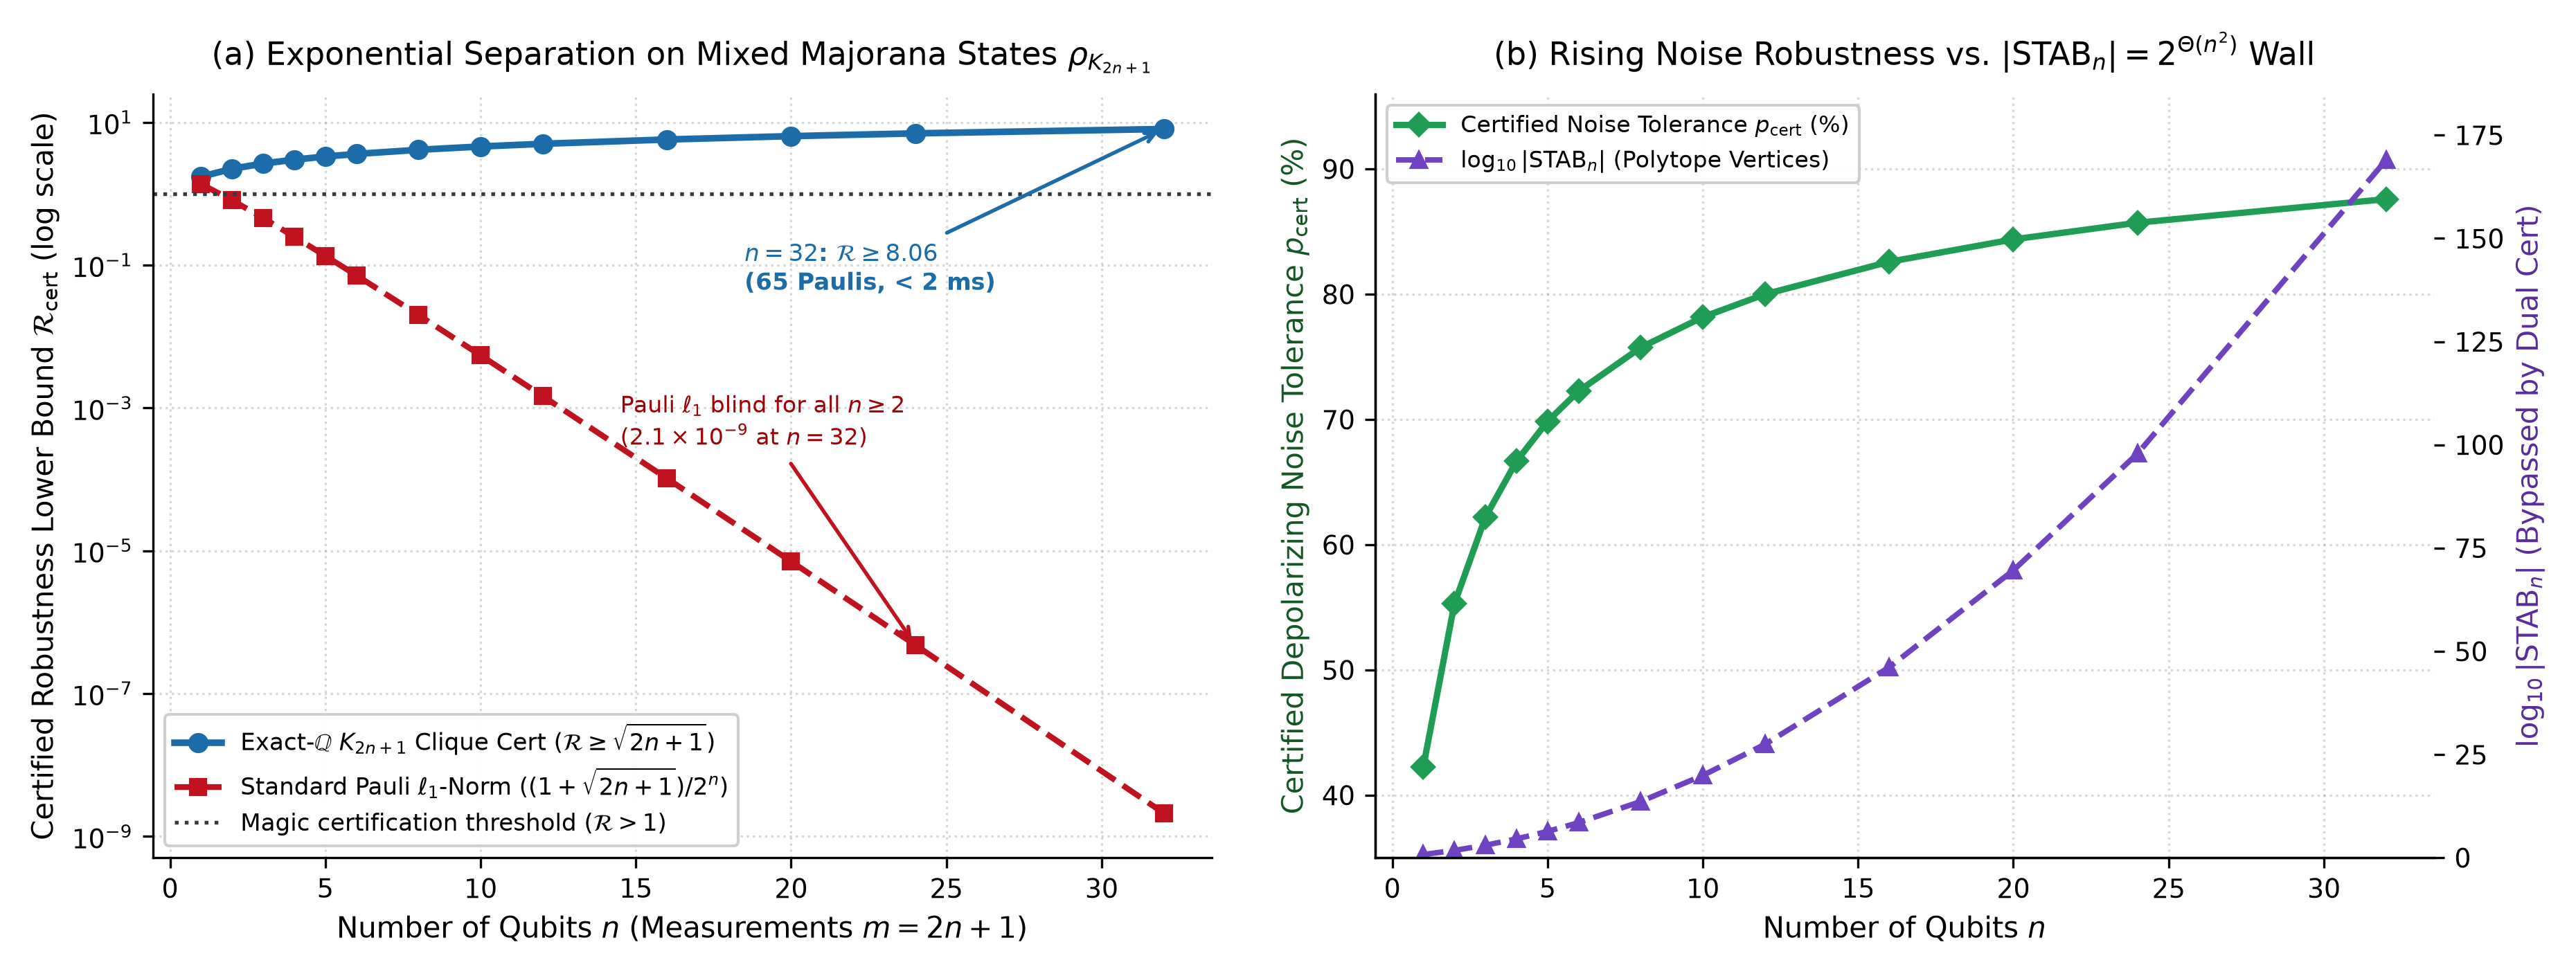
\includegraphics[width=\textwidth]{../figures/fig1_majorana_exponential_separation.png}
  \caption{(a)~Exponential separation between our exact-$\Q$ $K_{2n+1}$ clique certificate ($\RoM \ge \sqrt{2n+1}$) and the standard Pauli $\ell_1$-norm bound ($(1+\sqrt{2n+1})/2^n$, blind for all $n \ge 2$) on mixed Majorana states $\rho_{K_{2n+1}}$. (b)~Certified depolarizing noise tolerance rising to $87.6\%$ at $n=32$ alongside the bypassed $|\STAB_n| = 2^{\Theta(n^2)}$ vertex explosion ($\log_{10}|\STAB_{32}| = 168.95$).}
  \label{fig:fig1}
\end{figure}

\subsection{Experiment 3: Arbitrary-\texorpdfstring{$n$ $W$}{n W}-State Marginal Magic (\texorpdfstring{$n = 3\dots 50$}{n = 3..50}) and \texorpdfstring{$|\mathrm{CCZ}\rangle$}{|CCZ>}}
Figure~\ref{fig:fig2}(a) verifies Theorem~\ref{thm:w-state} from $n = 3$ ($\RoM \ge 5/3$, $p_{\mathrm{cert}} = 40.0\%$) through $n = 50$ ($\RoM \ge 26/25 = 1.04$, $p_{\mathrm{cert}} = 3.85\%$), using the same three weight-$\le 2$ Paulis $\{Z_0, X_0 X_1, Y_0 Y_2\}$ at every $n$; direct density-matrix partial trace for $n = 3, 4, 5$ confirms $\max_{i,j}|\rho^{(2)}_{W_n} - \rho_{\STAB_2}| < 10^{-15}$. On the 3-qubit Toffoli state $|\mathrm{CCZ}\rangle$, our 4-Pauli clique certifies $\RoM \ge 2$ ($p_{\mathrm{cert}} = 50.0\%$), strictly beating the 63-Pauli $\ell_1$-norm bound ($15/8 = 1.875$, $p_{\mathrm{cert}} = 46.7\%$) with $15.75\times$ fewer measurements.

\begin{figure}[t]
  \centering
  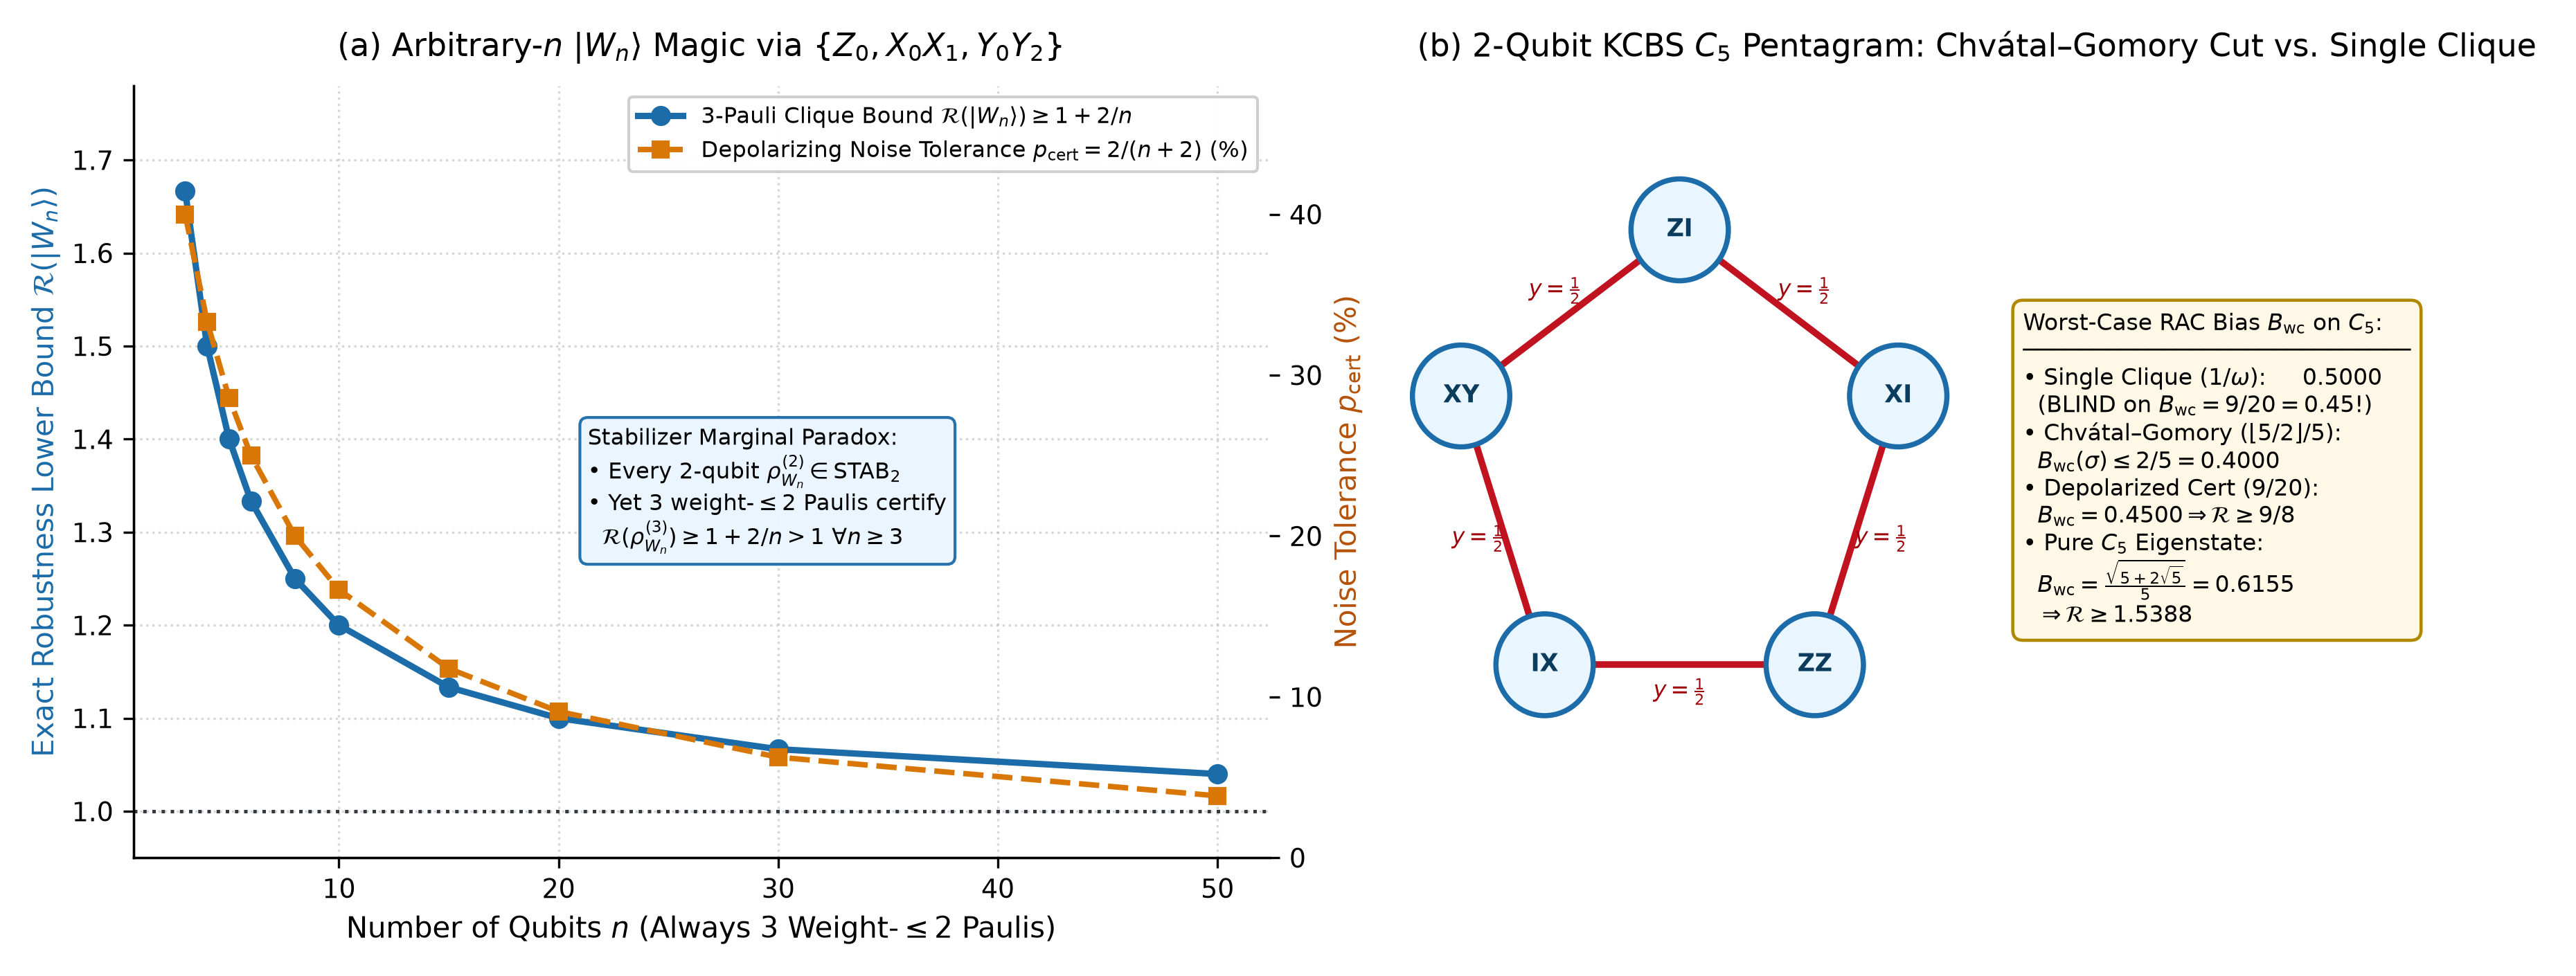
\includegraphics[width=\textwidth]{../figures/fig2_w_state_and_c5_pentagram.png}
  \caption{(a)~Exact 3-Pauli clique Robustness lower bound $\RoM(|W_n\rangle) \ge 1 + 2/n$ and noise tolerance $2/(n+2)$ for $n = 3\dots 50$, despite every 2-qubit marginal lying inside $\STAB_2$. (b)~2-qubit KCBS $C_5$ pentagram anticommutation graph with half-weight edge cliques ($y = 1/2$) whose Chv\'atal--Gomory floor $\lfloor 5/2 \rfloor = 2$ lowers the stabilizer RAC ceiling from $1/2$ to $2/5$, certifying magic on $B_{\mathrm{wc}} = 9/20$.}
  \label{fig:fig2}
\end{figure}

\subsection{Experiment 4: Strict 3-Tier Separation and 28-Attack Adversarial Suite}
Figure~\ref{fig:fig3}(a) visualizes all six fixed-witness separation benchmarks recorded in \Code{results/\allowbreak exp4\_\allowbreak hierarchy\_\allowbreak separation.\allowbreak json}: (i)~Tier~1 strictly beats Pauli $\ell_1$-norm on $K_5$ ($2.236$ vs $0.809$) and $|\mathrm{CCZ}\rangle$ ($2.000$ vs $1.875$); (ii)~Tier~2 Chv\'atal--Gomory rounding strictly beats Tier~1 on depolarized $C_5$ ($1.125$ vs $1.000$ blind) and boosts pure $C_5$ by $+25\%$ ($1.539$ vs $1.231$); and (iii)~on the \emph{fixed signed witness operators} $W_{\mathrm{FT6}}$ and $W_{\mathrm{FT8}}$, Tier~3 Signed Frustration strictly beats \emph{all} unsigned graph bounds evaluated on the fixed witness ($1.244$ vs $1.000$ on $W_{\mathrm{FT6}}$; $1.412$ vs $1.000$ on $W_{\mathrm{FT8}}$), while illustrating Proposition~\ref{prop:subset-dominance}: if individual Pauli expectations are instead subset-selected rather than summed into the fixed operator $W$, the embedded Tier~1 sub-cliques $C_3$ and $K_5$ attain $\sqrt{3} \approx 1.732$ and $\sqrt{5} \approx 2.236$ (plotted as hollow markers in Figure~\ref{fig:fig3}a). Note also that on the small 2-qubit benchmarks ($C_5$, $W_{\mathrm{FT6}}$, $W_{\mathrm{FT8}}$), the gray Pauli $\ell_1$-norm bar reflects full 15-Pauli tomography, whereas Pauli $\ell_1$-norm collapses exponentially on mixed states such as $\rho_{K_{2n+1}}$. Figure~\ref{fig:fig3}(b) displays exact-$\Q$ verification runtimes across all 9 certificates (all zero-enumeration checks complete in $\le 1.88\,\mathrm{ms}$). Finally, \Code{tests/\allowbreak test\_\allowbreak suite.py} attacks \Code{verify\_\allowbreak magic\_\allowbreak certificate\_\allowbreak exact} with \textbf{28 live adversarial forgeries} (14 algebraic/symplectic forgeries plus 14 canonical-parser and strict type-injection attacks covering \Code{float}, \Code{bool}, \Code{NaN}, decimals, unreduced \Code{"2/4"}, leading-zero \Code{"001"}, non-string dict keys, \Code{Decimal}, sets, and tuples), rejecting \textbf{28/28 attacks}.

\begin{figure}[t]
  \centering
  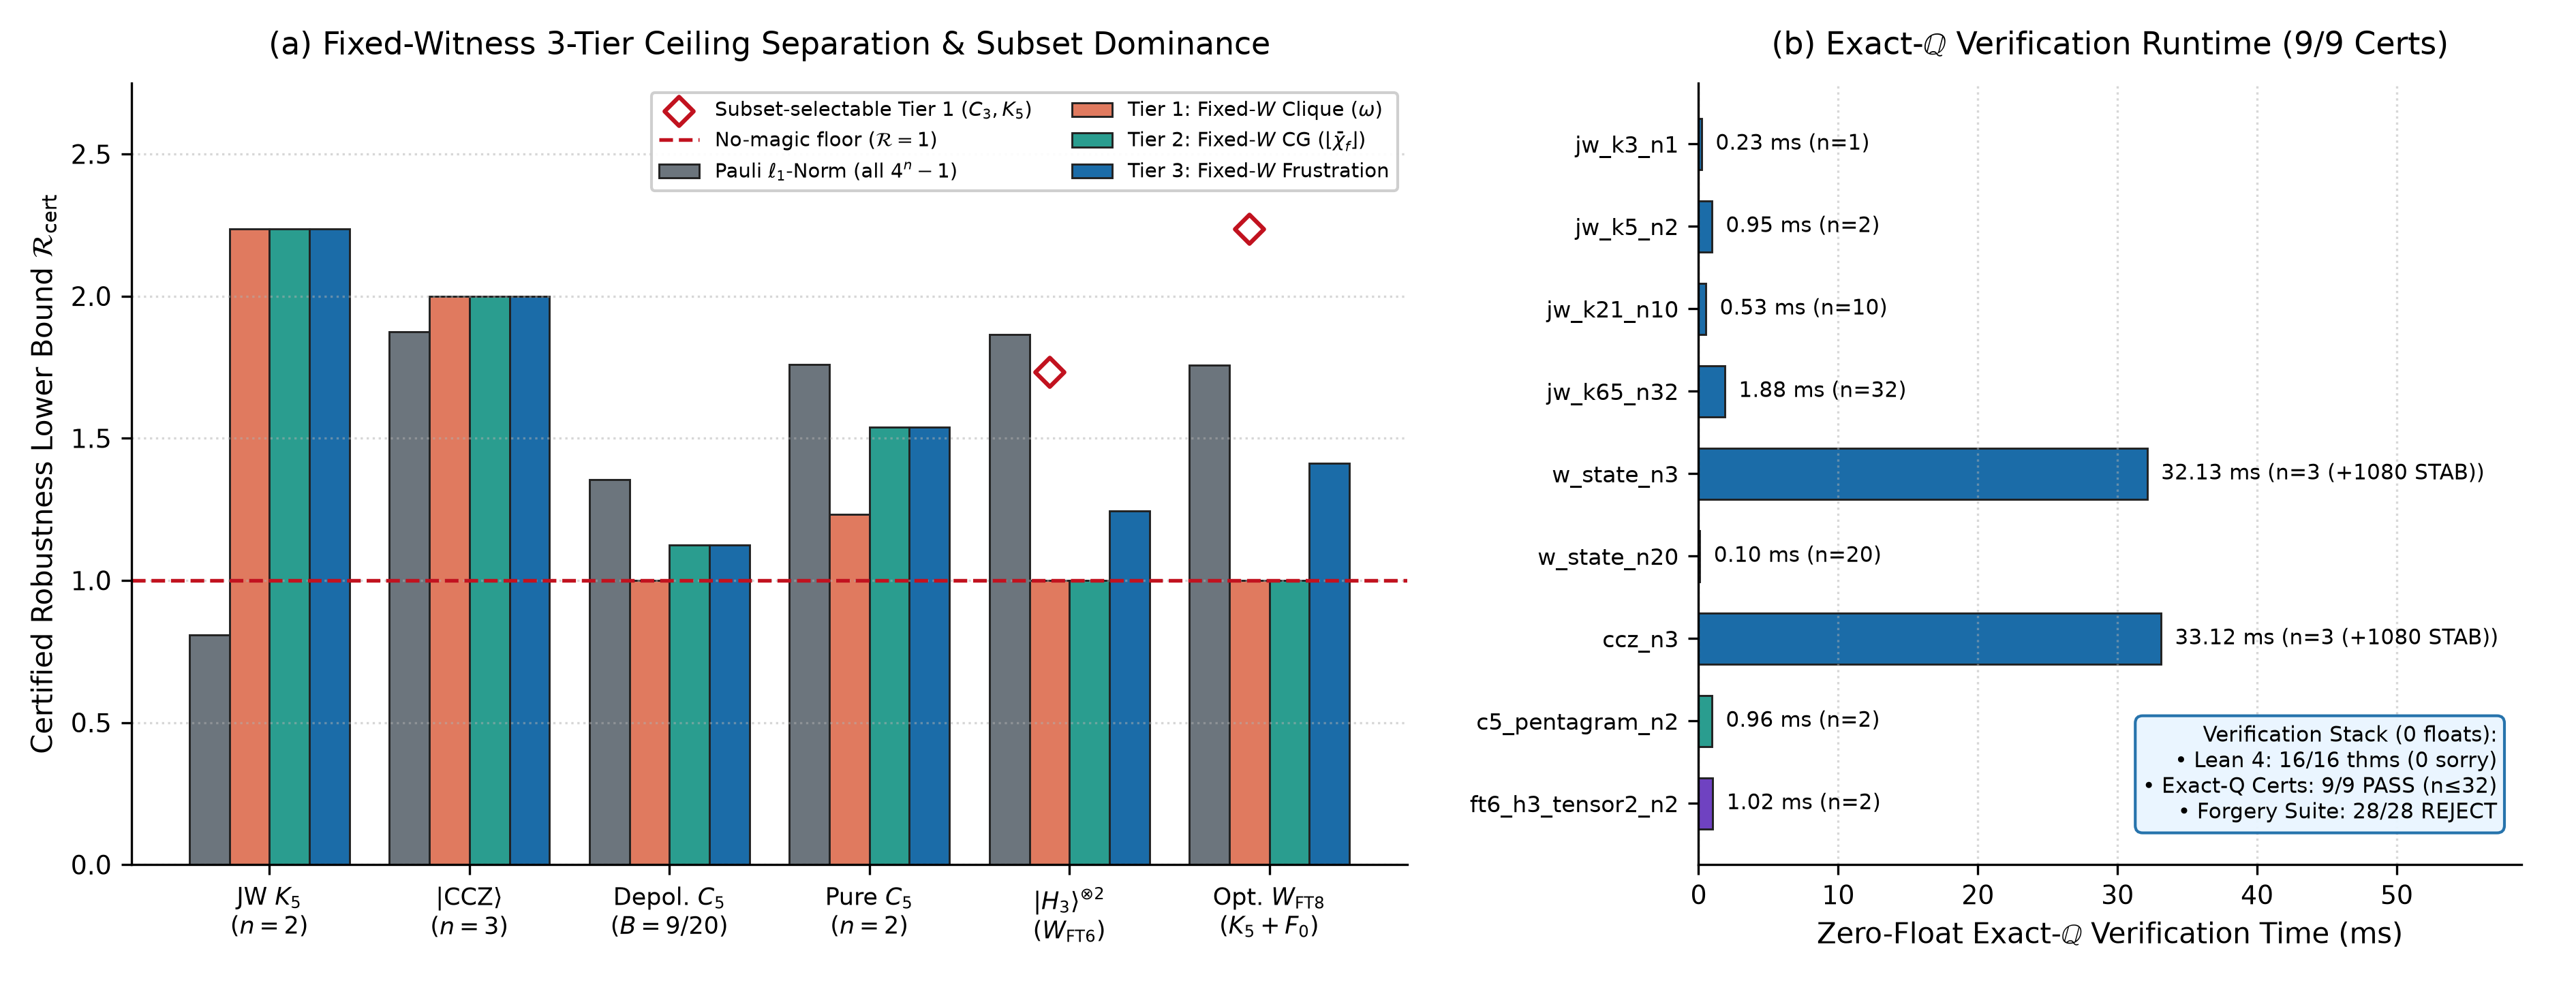
\includegraphics[width=\textwidth]{../figures/fig3_three_tier_hierarchy.png}
  \caption{(a)~Fixed-witness 3-tier ceiling separation across six multi-qubit magic benchmarks (Theorem~\ref{thm:hierarchy}): bars compare bounds on the \emph{fixed witness operator} $W$ (where unsigned graph ceilings on $W_{\mathrm{FT6}}$/$W_{\mathrm{FT8}}$ are blind at $\RoM_{\mathrm{cert}} = 1$), while diamond markers on $W_{\mathrm{FT6}}$/$W_{\mathrm{FT8}}$ show the strictly tighter subset-selectable Tier~1 sub-clique bounds ($\sqrt{3}, \sqrt{5}$) proved by Proposition~\ref{prop:subset-dominance}. (b)~Zero-float exact-$\Q$ verification runtimes for all 9 published certificates (including optional 1080-state $\STAB_3$ cross-checks on $n=3$ benchmarks).}
  \label{fig:fig3}
\end{figure}

\section{Limitations and Scope}
\label{sec:limitations}
Four clear scope boundaries apply: (1)~our dual verifier certifies \emph{valid lower bounds} on $\RoM(\rho)$ from a supplied atom decomposition and certified Pauli expectations—solving for the globally optimal atom decomposition on an arbitrary unknown $n$-qubit state still requires a classical primal/dual search heuristic (whose output is then audited with zero trust by our exact-$\Q$ verifier); (2)~global PSD quantum-state realizability ($\rho \succeq 0$) of the supplied \Code{state\_expectations} is an external physical assumption (established analytically as in Theorems~\ref{thm:majorana}--\ref{thm:hierarchy} or experimentally via tomography), not verified by the dual stabilizer-polytope checker; (3)~higher-order signed atoms beyond commuting triples (e.g., Mermin--Peres 9-observable contextual grids or 4-generator frustrated subgroups) can tighten Tier~3 further and are natural extensions of Definition~\ref{def:atoms}; and (4)~in laboratory deployments, finite-shot statistical confidence intervals on measured Pauli expectations replace the exact rational/radical expectation entries via conservative Clopper--Pearson or Hoeffding rational lower/upper intervals $[\mathrm{lo}_P, \mathrm{hi}_P]$, which our interval engine already accepts natively.

\section{Conclusion}
\label{sec:conclusion}
We have introduced a zero-enumeration, exact-$\Q$, Lean-4-mechanized hierarchy for certifying multi-qubit mixed-state non-stabilizerness and Robustness of Magic using anticommuting clique atoms, Chv\'atal--Gomory integer-floor cuts, and signed frustrated commuting triples. By bypassing the $2^{\Theta(n^2)}$ stabilizer-polytope wall completely, our framework certifies mixed-state magic up to $n = 32$ qubits in under $2\,\mathrm{ms}$, resolves the stabilizer-marginal problem for arbitrary $n$-qubit $W$-states using just three weight-$\le 2$ Paulis, and establishes strict separations across all three algebraic tiers.

\bibliographystyle{plain}
\bibliography{references}

\end{document}
